\documentclass[border=4pt]{standalone}
\usepackage{tikz}
\usepackage{amsmath,amssymb}
\usepackage{mathptmx}
\usetikzlibrary{arrows.meta,positioning,calc,shapes.geometric,decorations.pathreplacing,shadows,fadings,patterns}
\definecolor{cblue}{HTML}{1F4E9C}
\definecolor{cgold}{HTML}{D08C00}
\definecolor{cred}{HTML}{B5172E}
\definecolor{cgreen}{HTML}{1B7A3A}
\definecolor{cgrey}{HTML}{555555}
\definecolor{cpurple}{HTML}{5B2A86}
% oblique 3D cuboid: \cuboid{x}{y}{z}{dx}{dy}{dz}{colour}
\newcommand{\cuboid}[7]{%
  \fill[#7!55!white,draw=#7!60!black,line width=0.4pt] (#1,#2,#3+#6) -- ++(#4,0,0) -- ++(0,#5,0) -- ++(-#4,0,0) -- cycle;
  \fill[#7!80!black,draw=#7!60!black,line width=0.4pt] (#1+#4,#2,#3) -- ++(0,#5,0) -- ++(0,0,#6) -- ++(0,-#5,0) -- cycle;
  \fill[#7,draw=#7!60!black,line width=0.4pt] (#1,#2,#3) -- ++(#4,0,0) -- ++(0,0,#6) -- ++(-#4,0,0) -- cycle;}

\usepackage{graphicx}
\begin{document}
\begin{tikzpicture}[x={(1cm,0cm)},y={(0.4cm,0.3cm)},z={(0cm,1cm)},
  arr/.style={-{Stealth[length=2.2mm]},line width=0.7pt},
  lab/.style={font=\footnotesize,align=center}]
\node[font=\small\bfseries,anchor=west] at (-0.6,0,6.55) {(a) checks fixed on arrival};
% time axis
\draw[arr,cgrey] (-0.4,0,0) -- (7.6,0,0) node[below left,lab,cgrey] {arrival};
% candidates: a = 1, 3, 0.5, 6, 2, 12;  r = 8, 11, 14, 12, 14, 13 (eps = 1/2, theta = 0.01)
\foreach \n/\h/\r/\lab in {0/0.45/8/1,1/0.78/11/2,2/0.32/14/3,3/1.10/12/4,4/0.64/14/5,5/1.56/13/6}{
  \pgfmathsetmacro\xx{1.05*\n}
  \cuboid{\xx}{0}{0.05}{0.55}{0.55}{\h}{cblue}
  \node[lab] at (\xx+0.28,0,-0.32) {$a_{\lab}$};
  \pgfmathsetmacro\hh{0.12*\r}
  \cuboid{\xx+0.12}{0.12}{1.85}{0.3}{0.3}{\hh}{cgold}
  \node[lab,anchor=south] at (\xx+0.27,0.12,2.2+\hh) {$r_{\lab}{=}\r$};
  \draw[arr,cgrey,line width=0.5pt] (\xx+0.28,0,\h+0.12) -- (\xx+0.28,0.12,1.78);
}
% running total
\draw[cblue!60!black,line width=0.6pt,decorate,decoration={brace,amplitude=4pt,mirror}] (0,0,-0.62) -- (5.8,0,-0.62)
  node[midway,below=3pt,lab,black] {running total $S_{n}=a_{1}+\dots+a_{n}$, \ $u_{n}=\log(S_{n}/a_{1})$};
% the unknown future
\foreach \k in {0,1,2}{\draw[cgrey,dashed,line width=0.4pt] (6.35+0.4*\k,0,0.05) rectangle ++(0.3,0,0.5);}
\node[lab,cgrey] at (6.85,0,0.95) {future\\unknown};
% budget column: w = 0.5, 0.0659, 0.0089, 0.0254, 0.0064, 0.0139
\begin{scope}[shift={(8.75,0,0.05)}]
  \draw[line width=0.5pt,draw=black!70] (0,0,0) rectangle (0.75,0,4.6);
  \fill[cblue!70] (0,0,0) rectangle (0.75,0,2.3);
  \fill[cblue!50] (0,0,2.3) rectangle (0.75,0,2.603);
  \fill[cgold!70] (0,0,2.603) rectangle (0.75,0,2.644);
  \fill[cgreen!60] (0,0,2.644) rectangle (0.75,0,2.761);
  \fill[cpurple!50] (0,0,2.761) rectangle (0.75,0,2.790);
  \fill[cred!55] (0,0,2.790) rectangle (0.75,0,2.854);
  \draw[cred,line width=0.8pt] (-0.1,0,4.6) -- (0.85,0,4.6) node[right,lab,cred] {$1$};
  \node[lab,white] at (0.375,0,1.15) {$w_{1}$};
  \node[lab,anchor=west] at (0.85,0,2.58) {$w_{2},\dots,w_{6}$};
  \node[lab,anchor=north] at (0.375,0,-0.12) {$\sum_{n}w_{n}<1$\\whatever\\comes next};
\end{scope}
\node[lab,anchor=west,draw=gray!50,fill=white,rounded corners=2pt] at (-0.6,0,5.45)
 {$r_{n}=\Bigl\lceil\dfrac1L\log\dfrac{1}{\theta w_{n}}\Bigr\rceil,\qquad w_{n}=\dfrac{a_{n}/S_{n}}{2(1+u_{n})^{2}}$\\[2pt] runs computed from $a_{1},\dots,a_{n}$ only};
\node[anchor=south west,inner sep=0] at (11.1,0,-0.95) {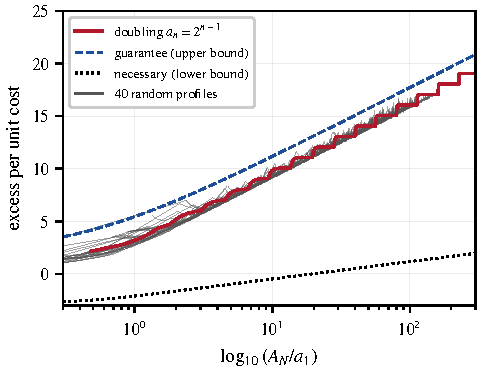
\includegraphics[width=9.0cm]{panel_online.pdf}};
\node[font=\small\bfseries,anchor=west] at (11.1,0,6.55) {(b) cost against dynamic range};
\end{tikzpicture}
\end{document}
